% answers.tex —— 1991 年·全国卷·文科 · 参考答案与详细解析片段
% 由 tools/generate_projects.py 依来源总账自 1991/1991_数学真题_全国文_试题.md + 1991/1991_数学真题_全国文_解析正文.md + 1991/1991_数学真题_全国文_答案要点.md 生成，勿手改（改源 MD 后重跑）


\begin{gktip}
本稿是根据固定源题面推导的非官方解析草稿。原件没有答案、解析或分值，不将推导结果标为官方答案。异人盲核尚未完成。第 24 题印文有双加号，依原样保留；第 24、26 题分别存在方向或主轴未定造成的多解，不擅自删去合法解。
\end{gktip}

\begin{answer}
\gksolhead{1}{}

\textbf{题目}：

已知 $\sin\alpha=\dfrac45$，并且 $\alpha$ 是第二象限的角，那么 $\tan\alpha$ 的值等于\mbox{（　　）}

（A）$-\dfrac43$　　（B）$-\dfrac34$　　（C）$\dfrac34$　　（D）$\dfrac43$

\Needspace{4\baselineskip}
\textbf{解析}

由 $\sin\alpha=4/5$ 及 $\alpha$ 在第二象限，得 $\cos\alpha=-3/5$，因此 $\tan\alpha=-4/3$，选 A。

\gkanswer{答案：A}

\end{answer}
\begin{answer}
\gksolhead{2}{}

\textbf{题目}：

焦点在 $(-1,0)$，顶点在 $(1,0)$ 的抛物线方程是\mbox{（　　）}

（A）$y^2=8(x+1)$　　（B）$y^2=-8(x+1)$

（C）$y^2=8(x-1)$　　（D）$y^2=-8(x-1)$

\Needspace{4\baselineskip}
\textbf{解析}

抛物线顶点为 $(1,0)$，焦点为 $(-1,0)$，焦点在顶点左侧，参数 $p=2$。标准式 $y^2=-4p(x-1)$，即 $y^2=-8(x-1)$，选 D。

\gkanswer{答案：D}

\end{answer}
\begin{answer}
\gksolhead{3}{}

\textbf{题目}：

点 $P(2,5)$ 关于直线 $x+y=0$ 的对称点的坐标是\mbox{（　　）}

（A）$(5,2)$　　（B）$(2,-5)$　　（C）$(-5,-2)$　　（D）$(-2,-5)$

\Needspace{4\baselineskip}
\textbf{解析}

关于直线 $y=-x$ 的反射将 $(x,y)$ 映为 $(-y,-x)$，故 $(2,5)$ 的对称点是 $(-5,-2)$，选 C。

\gkanswer{答案：C}

\end{answer}
\begin{answer}
\gksolhead{4}{}

\textbf{题目}：

函数 $y=\cos^4x-\sin^4x$ 的最小正周期是\mbox{（　　）}

（A）$\dfrac\pi2$　　（B）$\pi$　　（C）$2\pi$　　（D）$4\pi$

\Needspace{4\baselineskip}
\textbf{解析}

利用平方差，$\cos^4x-\sin^4x=(\cos^2x-\sin^2x)(\cos^2x+\sin^2x)=\cos2x$，其最小正周期为 $\pi$，选 B。

\gkanswer{答案：B}

\end{answer}
\begin{answer}
\gksolhead{5}{}

\textbf{题目}：

如果把两条异面直线看成“一对”，那么六棱锥的棱所在的 12 条直线中，异面直线共有\mbox{（　　）}

（A）12 对　　（B）24 对　　（C）36 对　　（D）48 对

\Needspace{4\baselineskip}
\textbf{解析}

六棱锥有 6 条底棱及 6 条侧棱，共 12 条棱所在直线。所有无序直线对有 $\binom{12}{2}=66$ 对；其中共面相交或平行的对数可按棱分类计数。将底面六边形记为 $A_1\dots A_6$、顶点记为 $S$：底棱直线间共有 $\binom62=15$ 对，均在底面内；6 条侧棱直线两两相交于 $S$，共有 $\binom62=15$ 对；每条底棱直线与侧棱直线共有 36 对，其中与它共面的两条侧棱所在直线各相交于端点，共有 $6\cdot2=12$ 对，其余 24 对异面。故异面直线对数为 24，选 B。

\gkanswer{答案：B}

\end{answer}
\begin{answer}
\gksolhead{6}{}

\textbf{题目}：

函数 $y=\sin\left(2x+\dfrac{5\pi}{2}\right)$ 的图象的一条对称轴的方程是\mbox{（　　）}

（A）$x=-\dfrac\pi2$　　（B）$x=-\dfrac\pi4$　　（C）$x=\dfrac\pi8$　　（D）$x=\dfrac{5\pi}4$

\Needspace{4\baselineskip}
\textbf{解析}

$\sin(2x+5\pi/2)=\cos2x$。函数 $\cos2x$ 的对称轴为 $x=k\pi/2$（$k\in\mathbb Z$），四个选项中只有 $x=-\pi/2$ 符合，选 A。

\gkanswer{答案：A}

\end{answer}
\begin{answer}
\gksolhead{7}{}

\textbf{题目}：

如果三棱锥 $S-ABC$ 的底面是不等边三角形，侧面与底面所成的二面角都相等，且顶点 $S$ 在底面的射影 $O$ 在 $\triangle ABC$ 内，那么 $O$ 是 $\triangle ABC$ 的\mbox{（　　）}

（A）垂心　　（B）重心　　（C）外心　　（D）内心

\Needspace{4\baselineskip}
\textbf{解析}

设棱锥高为 $h$，顶点在底面的射影为 $O$。对底面任一边，侧面与底面的二面角的正切等于 $h$ 除以 $O$ 到该边所在直线的距离。二面角都相等且 $h$ 固定，故 $O$ 到三边所在直线的距离相等。又 $O$ 在三角形内部，所以 $O$ 是内心，选 D。

\gkanswer{答案：D}

\end{answer}
\begin{answer}
\gksolhead{8}{}

\textbf{题目}：

已知 $\{a_n\}$ 是等比数列，且 $a_n>0$，$a_2a_4+2a_3a_5+a_4a_6=25$，那么 $a_3+a_5$ 的值等于\mbox{（　　）}

（A）5　　（B）10　　（C）15　　（D）20

\Needspace{4\baselineskip}
\textbf{解析}

\Needspace{5\baselineskip}
设等比数列公比为 $q$。有 $a_2a_4=a_3^2$、$a_3a_5=a_4^2$、$a_4a_6=a_5^2$，因而
\nopagebreak[4]
\[
a_2a_4+2a_3a_5+a_4a_6=(a_3+a_5)^2=25
\]
由 $a_n>0$ 得 $a_3+a_5>0$，所以 $a_3+a_5=5$，选 A。

\gkanswer{答案：A}

\end{answer}
\begin{answer}
\gksolhead{9}{}

\textbf{题目}：

已知函数 $y=\dfrac{6x+5}{x-1}$（$x\in\mathbb R$，$x\ne1$），那么它的反函数为\mbox{（　　）}

（A）$y=\dfrac{6x+5}{x-1}$（$x\in\mathbb R$，$x\ne1$）

（B）$y=\dfrac{x+5}{x-6}$（$x\in\mathbb R$，$x\ne6$）

（C）$y=\dfrac{x-1}{6x+5}$（$x\in\mathbb R$，$x\ne-\dfrac56$）

（D）$y=\dfrac{x-6}{x+5}$（$x\in\mathbb R$，$x\ne-5$）

\Needspace{4\baselineskip}
\textbf{解析}

令 $y=(6x+5)/(x-1)$，解得 $x=(y+5)/(y-6)$。原函数的值域不含 6，故反函数定义域为 $x\ne6$，反函数为 $y=(x+5)/(x-6)$，选 B。

\gkanswer{答案：B}

\end{answer}
\begin{answer}
\gksolhead{10}{}

\textbf{题目}：

从 4 台甲型和 5 台乙型电视机中任意取出 3 台，其中至少要有甲型与乙型电视机各 1 台，则不同的取法共有\mbox{（　　）}

（A）140 种　　（B）84 种　　（C）70 种　　（D）35 种

\Needspace{4\baselineskip}
\textbf{解析}

按甲型电视机取 1 台或 2 台分类：$\binom41\binom52+\binom42\binom51=40+30=70$ 种，选 C。

\gkanswer{答案：C}

\end{answer}
\begin{answer}
\gksolhead{11}{}

\textbf{题目}：

设甲、乙、丙是三个命题。如果甲是乙的必要条件；丙是乙的充分条件但不是乙的必要条件，那么\mbox{（　　）}

（A）丙是甲的充分条件，但不是甲的必要条件

（B）丙是甲的必要条件，但不是甲的充分条件

（C）丙是甲的充要条件

（D）丙不是甲的充分条件，也不是甲的必要条件

\Needspace{4\baselineskip}
\textbf{解析}

“甲是乙的必要条件”表示 $\text{乙}\Rightarrow\text{甲}$；“丙是乙的充分条件”表示 $\text{丙}\Rightarrow\text{乙}$。所以 $\text{丙}\Rightarrow\text{甲}$，即丙是甲的充分条件。又丙不是乙的必要条件，说明存在乙真而丙假的情形；此时甲真、丙假，故丙不是甲的必要条件。选 A。

\gkanswer{答案：A}

\end{answer}
\begin{answer}
\gksolhead{12}{}

\Needspace{5\baselineskip}
\textbf{题目}：

\nopagebreak[4]
\[
\lim_{n\to\infty}\left[n\left(1-\frac13\right)\left(1-\frac14\right)\left(1-\frac15\right)\cdots\left(1-\frac1{n+2}\right)\right]
\]

的值等于\mbox{（　　）}

（A）0　　（B）1　　（C）2　　（D）3

\Needspace{4\baselineskip}
\textbf{解析}

\Needspace{5\baselineskip}
括号内乘积为
\nopagebreak[4]
\[
n\prod_{k=3}^{n+2}\left(1-\frac1k\right)
=n\prod_{k=3}^{n+2}\frac{k-1}{k}
=\frac{2n}{n+2}\longrightarrow2
\]
选 C。

\gkanswer{答案：C}

\end{answer}
\begin{answer}
\gksolhead{13}{}

\textbf{题目}：

如果 $AC<0$ 且 $BC<0$，那么直线 $Ax+By+C=0$ 不通过\mbox{（　　）}

（A）第一象限　　（B）第二象限　　（C）第三象限　　（D）第四象限

\Needspace{4\baselineskip}
\textbf{解析}

由 $AC<0$、$BC<0$，$A$ 与 $B$ 同号且与 $C$ 异号。将方程整体乘以 $-1$（若需要）后可设 $A>0$、$B>0$、$C<0$。直线与两坐标轴的交点分别为 $(-C/A,0)$ 和 $(0,-C/B)$，都在正半轴上，所以直线不通过第四象限，选 D。

\gkanswer{答案：D}

\end{answer}
\begin{answer}
\gksolhead{14}{}

\textbf{题目}：

如果奇函数 $f(x)$ 在区间 $[3,7]$ 上是增函数且最小值为 5，那么 $f(x)$ 在区间 $[-7,-3]$ 上是\mbox{（　　）}

（A）增函数且最小值为 $-5$　　（B）增函数且最大值为 $-5$

（C）减函数且最小值为 $-5$　　（D）减函数且最大值为 $-5$

\Needspace{4\baselineskip}
\textbf{解析}

由于 $f$ 在 $[3,7]$ 上递增且最小值为 5，故 $f(3)=5$。奇函数在关于原点对称的区间 $[-7,-3]$ 上仍递增，且最大值在 $x=-3$ 处取得，为 $f(-3)=-f(3)=-5$，选 B。

\gkanswer{答案：B}

\end{answer}
\begin{answer}
\gksolhead{15}{}

\textbf{题目}：

圆 $x^2+2x+y^2+4y-3=0$ 上到直线 $x+y+1=0$ 的距离为 $\sqrt2$ 的点共有\mbox{（　　）}

（A）1 个　　（B）2 个　　（C）3 个　　（D）4 个

\Needspace{4\baselineskip}
\textbf{解析}

圆方程化为 $(x+1)^2+(y+2)^2=8$，圆心 $C=(-1,-2)$、半径 $2\sqrt2$。点到直线 $x+y+1=0$ 的距离为 $\sqrt2$，等价于点位于两条平行线 $x+y+1=\pm2$ 上。其中一条经过圆心，与圆交于 2 点；另一条到圆心的距离为 $2\sqrt2$，与圆相切于 1 点。共 3 点，选 C。

\gkanswer{答案：C}

\end{answer}
\begin{answer}
\gksolhead{16}{}

\textbf{题目}：

双曲线以直线 $x=-1$ 和 $y=2$ 为对称轴，如果它的一个焦点在 $y$ 轴上，那么它的另一个焦点的坐标是\underline{\hspace{7em}}。

\Needspace{4\baselineskip}
\textbf{解析}

双曲线中心为两条对称轴的交点 $(-1,2)$，焦点所在的横轴或纵轴必为其中一条。焦点在 $y$ 轴上，因此其横坐标为 0，只可能是 $(0,2)$；另一个焦点关于直线 $x=-1$ 对称，坐标为 $(-2,2)$。

\gkanswer{答案：$(-2,2)$}

\end{answer}
\begin{answer}
\gksolhead{17}{}

\textbf{题目}：

已知 $\sin x=\dfrac{\sqrt5-1}{2}$，则 $\sin 2\left(x-\dfrac\pi4\right)=$\underline{\hspace{6em}}。

\Needspace{4\baselineskip}
\textbf{解析}

\Needspace{5\baselineskip}
利用 $\sin(2x-\pi/2)=-\cos2x=2\sin^2x-1$，代入 $\sin x=(\sqrt5-1)/2$，得
\nopagebreak[4]
\[
2\left(\frac{\sqrt5-1}{2}\right)^2-1=2-\sqrt5
\]

\gkanswer{答案：$2-\sqrt5$}

\end{answer}
\begin{answer}
\gksolhead{18}{}

\textbf{题目}：

不等式 $\lg(x^2+2x+2)<1$ 的解集是\underline{\hspace{8em}}。

\Needspace{4\baselineskip}
\textbf{解析}

对数真数 $x^2+2x+2=(x+1)^2+1>0$ 恒成立。以 10 为底的对数函数递增，故原不等式等价于 $(x+1)^2+1<10$，即 $-4<x<2$。

\gkanswer{答案：$(-4,2)$}

\end{answer}
\begin{answer}
\gksolhead{19}{}

\textbf{题目}：

$(ax+1)^7$ 的展开式中，$x^3$ 的系数是 $x^2$ 的系数与 $x^4$ 的系数的等差中项。若实数 $a>1$，那么 $a=$\underline{\hspace{6em}}。

\Needspace{4\baselineskip}
\textbf{解析}

展开式中 $x^2,x^3,x^4$ 的系数依次为 $21a^2,35a^3,35a^4$。等差中项条件给出 $2\cdot35a^3=21a^2+35a^4$。由 $a>1$ 可除以 $7a^2$，得到 $5a^2-10a+3=0$。取大于 1 的根，$a=1+\sqrt{10}/5$。

\gkanswer{答案：$1+\dfrac{\sqrt{10}}5$}

\end{answer}
\begin{answer}
\gksolhead{20}{}

\textbf{题目}：

在长方体 $ABCD-A_1B_1C_1D_1$ 中，已知顶点 $A$ 上三条棱长分别是 $\sqrt2$、$\sqrt3$、2。如果对角线 $AC_1$ 与过点 $A$ 的相邻三个面所成的角分别是 $\alpha$、$\beta$、$\gamma$，那么

$\cos\alpha+\cos\beta+\cos\gamma=\underline{\hspace{7em}}$。

\Needspace{4\baselineskip}
\textbf{解析}

以三条棱为坐标轴方向，对角线向量长度为 $\sqrt{(\sqrt2)^2+(\sqrt3)^2+2^2}=3$。对三个坐标面，向量在面内的投影长度依次为 $\sqrt5$、$\sqrt6$、$\sqrt7$。直线与平面的夹角余弦等于向量面内投影长度除以向量长度，故所求为 $(\sqrt5+\sqrt6+\sqrt7)/3$。

\gkanswer{答案：$\dfrac{\sqrt5+\sqrt6+\sqrt7}{3}$}

\end{answer}
\begin{answer}
\gksolhead{21}{}

\textbf{题目}：

求函数 $y=\sin^2x+2\sin x\cos x+3\cos^2x$ 的最大值。

\Needspace{4\baselineskip}
\textbf{解析}

\Needspace{5\baselineskip}
化简得
\nopagebreak[4]
\[
y=2+\cos2x+\sin2x\le2+\sqrt{1^2+1^2}=2+\sqrt2
\]
当 $2x$ 取使 $\cos2x+\sin2x=\sqrt2$ 的值时等号成立，因此最大值为 $2+\sqrt2$。

\gkanswer{答案：$2+\sqrt2$}

\end{answer}
\begin{answer}
\gksolhead{22}{}

\textbf{题目}：

已知复数 $z=1+i$，求复数 $\dfrac{z^2-3z+6}{z+1}$ 的模和辐角的主值。

\Needspace{4\baselineskip}
\textbf{解析}

\Needspace{5\baselineskip}
代入 $z=1+i$，有 $z^2-3z+6=3-i$、$z+1=2+i$，所以
\nopagebreak[4]
\[
\frac{3-i}{2+i}=\frac{(3-i)(2-i)}5=1-i
\]
其模为 $\sqrt2$，辐角主值为 $-\pi/4$。

\gkanswer{答案：模为 $\sqrt2$，辐角的主值为 $-\dfrac\pi4$}

\end{answer}
\begin{answer}
\gksolhead{23}{}

\textbf{题目}：

如图，在三棱台 $ABC-A_1B_1C_1$ 中，已知 $AA_1\perp$ 底面 $ABC$，$A_1A=A_1B_1=B_1C_1=a$，$B_1B\perp BC$，且 $B_1B$ 和底面 $ABC$ 所成的角是 $45^\circ$，求这个棱台的体积。
\nopagebreak[4]
\begin{center}% 按 1991 全国文科原页重绘点线连接关系；投影仅示意，不表示比例。
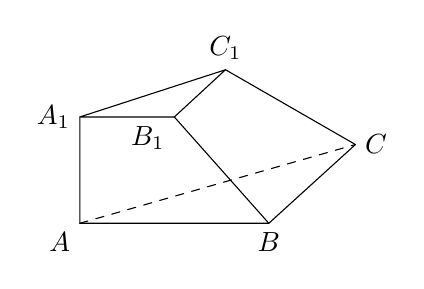
\begin{tikzpicture}[line join=round,line cap=round]
  \coordinate (A)  at (0,0);
  \coordinate (B)  at (2.4,0);
  \coordinate (C)  at (3.5,1.0);
  \coordinate (A1) at (0,1.35);
  \coordinate (B1) at (1.2,1.35);
  \coordinate (C1) at (1.85,1.95);
  \draw (A)--(B)--(C);
  \draw[dashed] (A)--(C);
  \draw (A)--(A1) (B)--(B1) (C)--(C1);
  \draw (A1)--(B1)--(C1)--cycle;
  \node[below left]  at (A)  {$A$};
  \node[below]       at (B)  {$B$};
  \node[right]       at (C)  {$C$};
  \node[left]        at (A1) {$A_1$};
  \node[below left]  at (B1) {$B_1$};
  \node[above]       at (C1) {$C_1$};
\end{tikzpicture}
\end{center}
\nopagebreak[4]
\Needspace{4\baselineskip}
\textbf{解析}

\Needspace{5\baselineskip}
设顶面与底面的相似比为 $k=A_1B_1/AB$。三棱台的对应侧棱延长后交于一点；由于 $AA_1$ 垂直底面，其交点在过 $A$ 的垂线上。$B_1B$ 在底面上的投影平行于 $AB$，且长度为 $(1-k)AB$。由 $B_1B\perp BC$，得 $AB\perp BC$。又 $B_1B$ 与底面成 $45^\circ$，故它的水平投影长度等于高 $AA_1=a$。同时 $A_1B_1=kAB=a$，于是 $kAB=(1-k)AB=a$，解得 $k=1/2$、$AB=2a$；由 $B_1C_1=kBC=a$ 得 $BC=2a$。底、顶面积分别为 $S_1=\tfrac12(2a)(2a)=2a^2$、$S_2=\tfrac12a^2$，高为 $a$。棱台体积为
\nopagebreak[4]
\[
V=\frac a3\left(S_1+S_2+\sqrt{S_1S_2}\right)=\frac76a^3
\]

\gkanswer{答案：$\dfrac76a^3$}

\end{answer}
\begin{answer}
\gksolhead{24}{}

\textbf{题目}：

设 $\{a_n\}$ 是等差数列，$b_n=\left(\dfrac12\right)^{a_n}$，已知：$b_1 + +b_2+b_3=\dfrac{21}{8}$，$b_1b_2b_3=\dfrac18$。求等差数列的通项 $a_n$。

\Needspace{4\baselineskip}
\textbf{解析}

\Needspace{5\baselineskip}
设 $a_n=a_1+(n-1)d$，则 $b_n=2^{-a_n}$ 为正项等比数列，公比 $r=2^{-d}>0$。由 $b_1b_2b_3=2^{-(a_1+a_2+a_3)}=2^{-3a_2}=1/8$，得 $a_2=1$、$b_2=1/2$。原页双加号按一元正号解释，和式为 $b_1+b_2+b_3$，故
\nopagebreak[4]
\[
\frac12\left(r^{-1}+1+r\right)=\frac{21}{8},\qquad r+r^{-1}=\frac{17}{4}
\]
解得 $r=4$ 或 $r=1/4$，即 $d=-2$ 或 $d=2$。因此通项有两种：$a_n=1-2(n-2)=5-2n$，或 $a_n=1+2(n-2)=2n-3$。条件对 $b_1,b_3$ 对称，不能确定公差的符号。

\gkanswer{答案：$a_n=2n-3$ 或 $a_n=5-2n$}

\end{answer}
\begin{answer}
\gksolhead{25}{}

\textbf{题目}：

设 $a>0$，$a\ne1$，解关于 $x$ 的不等式：$a^{x^4-2x^2}>\left(\frac1a\right)^{a^2}$。

\Needspace{4\baselineskip}
\textbf{解析}

若 $a>1$，指数函数递增，不等式化为 $x^4-2x^2>-a^2$，即 $u^2-2u+a^2>0$，其中 $u=x^2\ge0$。该二次式判别式 $4(1-a^2)<0$ 且首项系数为正，故对所有 $x\in\mathbb R$ 成立。

\Needspace{5\baselineskip}
若 $0<a<1$，指数函数递减，不等号反向，得到 $u^2-2u+a^2<0$。两根为 $u_\pm=1\pm\sqrt{1-a^2}$，且 $0<u_-<u_+$，所以 $u_-<x^2<u_+$，即
\nopagebreak[4]
\[
x\in\left(-\sqrt{u_+},-\sqrt{u_-}\right)\cup\left(\sqrt{u_-},\sqrt{u_+}\right)
\]
端点不包含，因为原不等式为严格不等式。

\gkanswer{答案：若 $a>1$，$x\in\mathbb R$；若 $0<a<1$，$x\in\left(-\sqrt{1+\sqrt{1-a^2}},-\sqrt{1-\sqrt{1-a^2}}\right)\cup\left(\sqrt{1-\sqrt{1-a^2}},\sqrt{1+\sqrt{1-a^2}}\right)$。}

\end{answer}
\begin{answer}
\gksolhead{26}{}

\textbf{题目}：

已知椭圆的中心在坐标原点 $O$，焦点在坐标轴上，直线 $y=x+1$ 与该椭圆相交于 $P$ 和 $Q$，且 $OP\perp OQ$，$|PQ|=\dfrac{\sqrt{10}}2$，求椭圆的方程。

\Needspace{4\baselineskip}
\textbf{解析}

\Needspace{5\baselineskip}
设椭圆方程为 $x^2/U+y^2/V=1$，其中 $U,V>0$，其主轴沿坐标轴。将 $y=x+1$ 代入，交点的横坐标 $x_1,x_2$ 满足
\nopagebreak[4]
\[
\left(\frac1U+\frac1V\right)x^2+\frac2Vx+\left(\frac1V-1\right)=0
\]
由韦达定理，$x_1+x_2=-2U/(U+V)$、$x_1x_2=U(1-V)/(U+V)$。又 $OP\perp OQ$ 给出 $x_1x_2+(x_1+1)(x_2+1)=0$，化简为 $U+V=2UV$。

\Needspace{5\baselineskip}
此外，$|PQ|^2=2(x_1-x_2)^2$。将上述韦达关系代入，得
\nopagebreak[4]
\[
|PQ|^2=\frac{8UV(U+V-1)}{(U+V)^2}=\frac{4(U+V-1)}{U+V}
\]
\Needspace{5\baselineskip}
由 $|PQ|^2=10/4=5/2$，解得 $U+V=8/3$，再由 $U+V=2UV$ 得 $UV=4/3$。因此 $U,V$ 是方程 $t^2-\tfrac83t+\tfrac43=0$ 的两根，即 $\{U,V\}=\{2,2/3\}$。原题没有说明长轴平行 $x$ 轴还是 $y$ 轴，所以两种互换方程都满足条件：
\nopagebreak[4]
\[
\frac{x^2}{2}+\frac{y^2}{2/3}=1
\qquad\text{\text{或}}\qquad
\frac{x^2}{2/3}+\frac{y^2}{2}=1
\]
不应在没有额外方向条件时只保留其中一种。

\gkanswer{答案：题设未确定长轴方向，方程有两种：$\frac{x^2}{2}+\frac{y^2}{2/3}=1$ 或 $\frac{x^2}{2/3}+\frac{y^2}{2}=1$。}

\end{answer}